\documentclass[a4paper,11pt]{article}
\usepackage[a4paper,margin=2.5cm]{geometry}
\usepackage[T1]{fontenc}
\usepackage{textcomp}
\usepackage{graphicx}
\usepackage{booktabs}
\usepackage{longtable}
\usepackage{tikz}
\usetikzlibrary{shapes.geometric,arrows.meta,positioning,fit,backgrounds}
\usepackage{listings}
\usepackage{xcolor}
\usepackage[hidelinks]{hyperref}
\usepackage{caption}
\usepackage{parskip}

\definecolor{pinpilotblue}{RGB}{30,100,200}
\definecolor{espcol}{RGB}{220,235,255}
\definecolor{sensorcol}{RGB}{220,255,220}
\definecolor{actuatorcol}{RGB}{255,235,200}
\definecolor{displaycol}{RGB}{255,220,255}

\hypersetup{colorlinks=false}

\title{\textbf{\color{pinpilotblue}PinPilot Wiring Documentation}\\[0.5em]\large Smart Farm Node\\[0.3em]\normalsize Board: ESP32 DevKit (WROOM-32)}
\author{Generated by \textbf{PinPilot} (IBM Bob 2.0 Hackathon)}
\date{\today}

\begin{document}
\maketitle
\tableofcontents
\newpage

\section{Project Summary}

This document describes the wiring, pin assignment, bus configuration, and LVGL dashboard layout for the \textbf{Smart Farm Node} demo project. The target board is the \textbf{ESP32 DevKit (WROOM-32)}.

\begin{center}
\begin{tabular}{ll}
\toprule
\textbf{Property} & \textbf{Value} \\
\midrule
Board & ESP32 DevKit (WROOM-32) \\
Components & 5 \\
Buses & i2c0, spi0 \\
WiFi enabled & Yes \\
Serial logging & Yes \\
LVGL version & 9.2.2 \\
RAM usage & 29.0\% \\
Flash usage & 41.2\% \\
\bottomrule
\end{tabular}
\end{center}

\section{Block Diagram}

\begin{center}
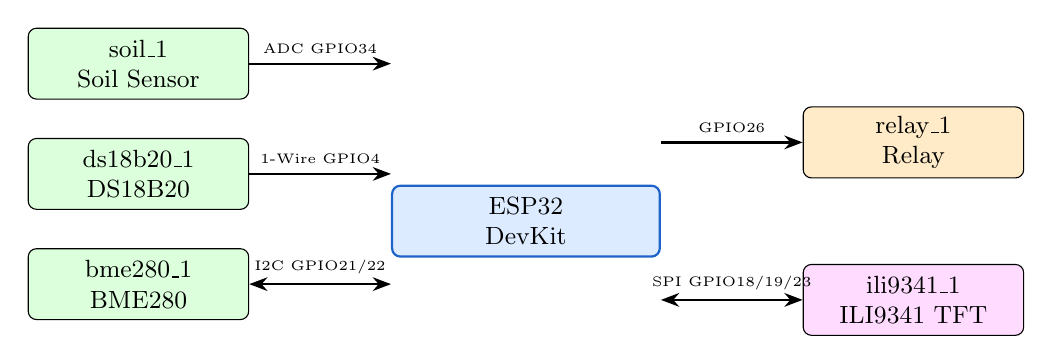
\begin{tikzpicture}[
  node distance=0.6cm and 1.8cm,
  every node/.style={font=\small},
  box/.style={draw, rounded corners=3pt, minimum width=2.8cm, minimum height=0.9cm, align=center},
  esp/.style={box, fill=espcol, draw=pinpilotblue, thick, minimum width=3.4cm},
  sensor/.style={box, fill=sensorcol},
  actuator/.style={box, fill=actuatorcol},
  display/.style={box, fill=displaycol},
  arr/.style={-{Stealth}, thick},
  barr/.style={{Stealth}-{Stealth}, thick},
]
  % ESP32 centre
  \node[esp] (esp) {ESP32\\DevKit};
  % Sensors — left column
  \node[sensor, left=of esp, yshift=2.0cm] (soil) {soil\_1\\Soil Sensor};
  \node[sensor, left=of esp, yshift=0.6cm] (ds)   {ds18b20\_1\\DS18B20};
  \node[sensor, left=of esp, yshift=-0.8cm] (bme)  {bme280\_1\\BME280};
  % Actuator — right top
  \node[actuator, right=of esp, yshift=1.0cm] (relay) {relay\_1\\Relay};
  % Display — right bottom
  \node[display, right=of esp, yshift=-1.0cm] (tft) {ili9341\_1\\ILI9341 TFT};
  % Arrows
  \draw[arr] (soil.east)  -- node[above,font=\tiny]{ADC GPIO34}  (esp.west |- soil.east);
  \draw[arr] (ds.east)    -- node[above,font=\tiny]{1-Wire GPIO4} (esp.west |- ds.east);
  \draw[barr] (bme.east)  -- node[above,font=\tiny]{I2C GPIO21/22} (esp.west |- bme.east);
  \draw[arr] (esp.east |- relay.west) -- node[above,font=\tiny]{GPIO26} (relay.west);
  \draw[barr] (esp.east |- tft.west)  -- node[above,font=\tiny]{SPI GPIO18/19/23} (tft.west);
\end{tikzpicture}
\end{center}

\section{Component List}

\begin{longtable}{llll}
\toprule
\textbf{Instance ID} & \textbf{Catalog Name} & \textbf{Interface} & \textbf{GPIO Summary} \\
\midrule
\endhead
\bottomrule
\endfoot
soil\_1 & Capacitive Soil Moisture Sensor v1.2 & ADC & AOUT=34 \\
ds18b20\_1 & DS18B20 & 1-Wire & DQ=4 \\
bme280\_1 & BME280 & I2C 0x76 & SDA=21, SCL=22 \\
relay\_1 & Relay Module (single channel, 5V coil) & GPIO & IN=26 \\
ili9341\_1 & ILI9341 2.8" TFT (SPI) & SPI & MOSI=23, MISO=19, SCK=18, CS=27, DC=16, RESET=17 \\
\end{longtable}

\section{Wiring Table}

\begin{longtable}{p{2.5cm}p{2cm}p{1.5cm}p{7.5cm}}
\toprule
\textbf{Instance} & \textbf{Pin} & \textbf{GPIO} & \textbf{GPIO Notes} \\
\midrule
\endhead
\bottomrule
\endfoot
soil\_1 & AOUT & 34 & Input-only. No internal pull-up or pull-down. ADC1 channel 6. \\
\midrule
ds18b20\_1 & DQ & 4 & ADC2 channel 0 --- unavailable when WiFi is active. \\
\midrule
bme280\_1 & SDA & 21 & Default I2C SDA. \\
bme280\_1 & SCL & 22 & Default I2C SCL. \\
\midrule
relay\_1 & IN & 26 & ADC2 channel 9 --- unavailable when WiFi is active. DAC channel 2. \\
\midrule
ili9341\_1 & MOSI & 23 & Default VSPI MOSI. \\
ili9341\_1 & MISO & 19 & Default VSPI MISO. \\
ili9341\_1 & SCK & 18 & Default VSPI SCK. \\
ili9341\_1 & CS & 27 & ADC2 channel 7 --- unavailable when WiFi is active. \\
ili9341\_1 & DC & 16 & Default UART2 RX. Good general-purpose I/O. \\
ili9341\_1 & RESET & 17 & Default UART2 TX. Good general-purpose I/O. \\
\midrule
\end{longtable}

\section{Pin Map}

All ESP32 GPIO assignments at a glance:

\begin{center}
\begin{tabular}{rll}
\toprule
\textbf{GPIO} & \textbf{Assigned To} & \textbf{Pin / Function} \\
\midrule
4 & ds18b20\_1 & DQ \\
16 & ili9341\_1 & DC \\
17 & ili9341\_1 & RESET \\
18 & ili9341\_1 & SCK \\
19 & ili9341\_1 & MISO \\
21 & bme280\_1 & SDA \\
22 & bme280\_1 & SCL \\
23 & ili9341\_1 & MOSI \\
26 & relay\_1 & IN \\
27 & ili9341\_1 & CS \\
34 & soil\_1 & AOUT \\
\bottomrule
\end{tabular}
\end{center}

\section{Bus Configuration}

\subsection{I2C (i2c0)}
\begin{tabular}{ll}
\toprule
\textbf{Parameter} & \textbf{Value} \\
\midrule
SDA & GPIO 21 \\
SCL & GPIO 22 \\
Frequency & 400\,kHz \\
\midrule
bme280\_1 address & 0x76 (118) \\
\bottomrule
\end{tabular}

\subsection{SPI (spi0)}
\begin{tabular}{ll}
\toprule
\textbf{Parameter} & \textbf{Value} \\
\midrule
MOSI & GPIO 23 \\
MISO & GPIO 19 \\
SCK  & GPIO 18 \\
Frequency & 40\,MHz \\
CS (ili9341\_1) & GPIO 27 \\
\bottomrule
\end{tabular}

\section{Component Notes}

\subsection{soil\_1 --- Capacitive Soil Moisture Sensor v1.2}

Must use an ADC1 pin (GPIO32--36, 39) when WiFi is enabled --- ADC2 pins are disabled by the WiFi driver. Output does NOT reach 3.3V: typical range is \~{}2.5--2.9V in dry air and \~{}1.0--1.5V submerged in water at 3.3V supply. Always calibrate --- thresholds vary by sensor unit and PCB revision. Some clones use an NE555 oscillator that requires a 5V supply to function correctly; if the sensor output looks wrong at 3.3V, try powering VCC from 5V.

\subsection{ds18b20\_1 --- DS18B20}

Requires a 4.7k\ensuremath{\Omega} pull-up resistor between DQ and VCC --- the ESP32 internal pull-up is too weak for reliable 1-Wire communication. The DallasTemperature library wraps OneWire for convenience; both must be in lib\_deps. Temperature conversion at 12-bit resolution takes up to 750 ms --- do not use delay(); use non-blocking requestTemperatures() + isConversionComplete().

\subsection{bme280\_1 --- BME280}

3.3V device --- do not connect to 5V supply. SDO to GND selects address 0x76 (default); SDO to VCC selects 0x77. Always pass the address explicitly to begin() --- the Adafruit library defaults to 0x77 but generic modules typically use 0x76. Many cheap modules are actually BMP280 (no humidity sensor): verify by checking the chip ID returned by begin(). The breakout board usually includes pull-ups on SDA/SCL; a second device on the bus does not need more pull-ups.

\subsection{relay\_1 --- Relay Module (single channel, 5V coil)}

The coil requires 5V --- power from the DevKit's 5V (VIN) pin. Most modules are ACTIVE LOW: writing LOW energizes the relay, HIGH releases it. 3.3V compatibility warning: 5V active-LOW opto modules may not switch OFF reliably when the ESP32 drives the IN pin HIGH at 3.3V. Safe options: (1) remove the JD-VCC jumper and power VCC=3.3V / JD-VCC=5V separately so the opto input is 3.3V-referenced; (2) use a relay module rated for 3.3V coil; (3) add a transistor driver (e.g. 2N2222 + 1k\ensuremath{\Omega} base resistor). Firmware tip: write HIGH to the IN pin before calling pinMode(OUTPUT) to prevent the relay from clicking at boot when the GPIO floats low during initialization.

\subsection{ili9341\_1 --- ILI9341 2.8" TFT (SPI)}

Configure TFT\_eSPI exclusively through build\_flags in platformio.ini --- never edit files inside .pio/libdeps/. Required build flags: -D USER\_SETUP\_LOADED -D ILI9341\_DRIVER -D TFT\_MOSI=23 -D TFT\_SCLK=18 -D TFT\_CS=<pin> -D TFT\_DC=<pin> -D TFT\_RST=<pin> -D SPI\_FREQUENCY=40000000. Use LVGL v9 API only (NOT v8). Use a partial draw buffer (\~{}1/10 screen = 320*24*2 = \~{}15 KB).

\section{LVGL Dashboard Layout}

Driver: \texttt{ili9341}\quad Display instance: \texttt{ili9341\_1}

Firmware built with \textbf{LVGL v9.2.2} (TFT\_eSPI back-end). RAM usage: \textbf{29.0\%}, Flash usage: \textbf{41.2\%}.

\begin{longtable}{p{2.8cm}p{1.5cm}p{3.5cm}rrrrrr}
\toprule
\textbf{Widget ID} & \textbf{Type} & \textbf{Binding} & \textbf{X} & \textbf{Y} & \textbf{W} & \textbf{H} & \textbf{Min} & \textbf{Max} \\
\midrule
\endhead
\bottomrule
\endfoot
moisture\_arc & arc & soil\_1.moisture & 10 & 40 & 100 & 100 & 0 & 100 \\
temp\_label & value & bme280\_1.temperature & 160 & 20 & — & — & — & — \\
soil\_temp\_label & value & ds18b20\_1.temperature & 160 & 80 & — & — & — & — \\
moisture\_chart & chart & soil\_1.moisture & 0 & 160 & 320 & 70 & 0 & 100 \\
\end{longtable}

\subsection{Dashboard Canvas (320\texttimes240)}

\begin{center}
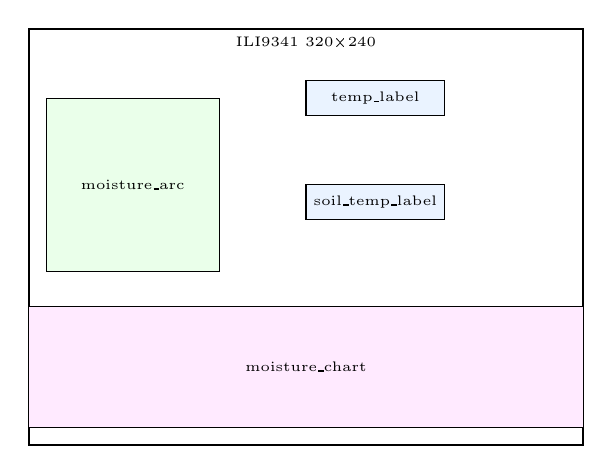
\begin{tikzpicture}[scale=0.022, every node/.style={font=\tiny}]
  % Screen border 320x240
  \draw[thick] (0,0) rectangle (320,240);
  \node at (160,232) {ILI9341 320\texttimes240};
  \draw[fill=sensorcol!60] (10,100) rectangle (110,200);
  \node[align=center] at (60.0,150.0) {moisture\_arc};
  \draw[fill=espcol!60] (160,190) rectangle (240,210);
  \node at (200,200) {temp\_label};
  \draw[fill=espcol!60] (160,130) rectangle (240,150);
  \node at (200,140) {soil\_temp\_label};
  \draw[fill=displaycol!60] (0,10) rectangle (320,80);
  \node[align=center] at (160.0,45.0) {moisture\_chart};
\end{tikzpicture}
\end{center}

\section{Firmware Build Result}

\begin{center}
\begin{tabular}{ll}
\toprule
\textbf{Item} & \textbf{Value} \\
\midrule
LVGL version & 9.2.2 \\
TFT\_eSPI version & 2.5.43 \\
Build status & \textcolor{green!60!black}{\textbf{SUCCESS}} \\
RAM usage & 29.0\% \\
Flash usage & 41.2\% \\
\bottomrule
\end{tabular}
\end{center}

\end{document}
